\documentclass{article}
\usepackage{graphicx} % Required for inserting images
\usepackage{hyperref}
\usepackage{physics}
\usepackage{tikz}
\usetikzlibrary{angles, quotes}
\usepackage{textcomp}
\usepackage{amsmath}
\usepackage{quantikz}




\title{IndependentStudy}
\author{Matthew Robson}
\date{September 2025}


\newcommand{\compconj}[1]{%
  \overline{#1}%
}


\begin{document}

\maketitle

\section{Classical Information and Computation} %%%%%%%%%%%%%%%%%%%%%%%%%%%%%%%%%%%%%%%%%%%%

This entire section was covered by my work in Digital Electronics. If you wish to view an example of my completed work, you can access it though my \href{https://github.com/orange314159}{Git} repository. 

\section{One Quantum Bit} %%%%%%%%%%%%%%%%%%%%%%%%%%%%%%%%%%%%%%%%%%%%

\subsection{Qubit Touchdown} %%%%%%%%%%%%%%%%%%%%%%%%%%%%%%%%%%%%%%%%%%%%

Qubit Touchdown is a game designed to introduce the player to the basics of a quantum bit.

\subsection{Superposition}

Qubits are represented as a super position of $\ket{0}$ and $\ket{1}$. $\ket{0}$ corresponds to the vector $(0,0,1)$ and $\ket{1}$ corresponds to the vector $(0,0,-1)$. Here are the definitions of some commonly used kets:
\begin{itemize}
    \item $\ket{+}  = \frac{1}{\sqrt{2}}(\ket{0} + \ket{1})$
    \item $\ket{-}  = \frac{1}{\sqrt{2}}(\ket{0} - \ket{1})$
    \item $\ket{i}  = \frac{1}{\sqrt{2}}(\ket{0} + i\ket{1})$
    \item $\ket{-i} = \frac{1}{\sqrt{2}}(\ket{0} - i\ket{1})$
\end{itemize}
Qubits can be defined by some vector $\ket{\psi}$ on the Bloch Sphere.\\
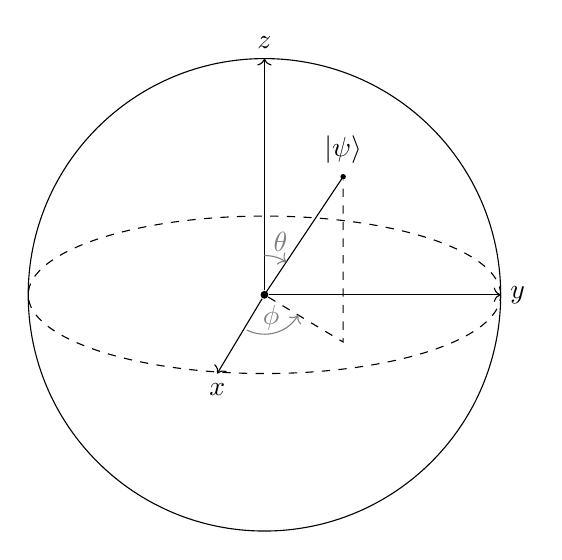
\begin{tikzpicture}

  % Define radius
  \def\r{3}

  % Bloch vector
  \draw (0,0) node[circle, fill, inner sep=1] (orig) {} -- (\r/3,\r/2)
    node[circle, fill, inner sep=0.7, label=above:$\ket{\psi}$] (a) {};
  \draw[dashed] (orig) -- (\r/3, -\r/5) node (phi) {} -- (a);

  % Sphere
  \draw (orig) circle (\r);
  \draw[dashed] (orig) ellipse (\r{} and \r/3);

  % Axes
  \draw[->] (orig) -- ++(-\r/5, -\r/3) node[below] (x1) {$x$};
  \draw[->] (orig) -- ++(\r, 0) node[right] (x2) {$y$};
  \draw[->] (orig) -- ++(0, \r) node[above] (x3) {$z$};

  % Angles
  \pic [draw=gray, text=gray, ->, "$\phi$"] {angle = x1--orig--phi};
  \pic [draw=gray, text=gray, <-, "$\theta$", angle eccentricity=1.4] {angle = a--orig--x3};

\end{tikzpicture} %% first bloch sphere
\\ 
A common function used in quantum computing is the norm-square. The norm-square is defined as $|x|^2 = xx^* | x* = \compconj{x}$.

\subsection{Measurement}

A qubit is most commonly measured in the z basis, as to give a $\ket{1}$ or $\ket{0}$. In the superposition $\frac{1}{\sqrt{2}}(\ket{1}+e^{\frac{i\pi}{6}}\ket{0})$ the probability of measuring a 1 is equivalent to the norm-square of the coefficient of $\ket{1}$, as for the probability of measuring a 0. In this example, that would mean $p(\ket{0}) = |\frac{1}{\sqrt{2}}|^{2} = \frac{1}{2}$, and $p(\ket{1}) = |\frac{e^{\frac{i\pi}{6}}}{\sqrt{2}}|^{2} = \frac{1}{2}$. In the case where the probabilities of measuring in a basis would result in a sum of greater than one, there is a normalization constant placed in front to set the total probability to one. In our example, the $\frac{1}{\sqrt{2}}$ is the normalization constant. Measurement can be done in any basis, that is, between two positions that oppose each other on the Bloch Sphere. 

\subsection{Bloch Sphere Mapping}

A global phase in the form of $e^{i\theta}$ may be placed in front of the superposition, but this phase will not impact the probability of measurement in any basis. Given some quantum state $\ket{\psi}$, this can be written as some $\ket{\psi} = \alpha\ket{0}+\beta\ket{1}| \abs{\alpha}^2+\abs{\beta}^2=1$. This means that $\alpha$ and $\beta$ can be represented as cosine and sine, as in $\alpha = \cos{\frac{\theta}{2}}, \beta = e^{i\phi}\sin{\frac{\theta}{2}}$, explaining the above Bloch Sphere figure. In order to further understand this position, in some cases $\ket{\phi}$ will be represented using Cartesian coordinates (x,y,z). These coordinates are defined by the following set of equations. 
\begin{itemize}
    \item $x = \sin{\theta}\cos{\phi}$
    \item $y = \sin{\theta}\sin{\phi}$
    \item $z = \cos{\theta}$
\end{itemize}
As an additional note, by measuring a qubit, you collapse the state to one location, but if you were to measure the same qubit in alternating bases, you would be able to measure consecutive p (0.5) events. Ex. Alternate measuring in the $\ket{0}, \ket{1}$ basis, then in the $\ket{+}, \ket{-}$ basis. 

\subsection{Physical Qubits}

There are many ways in which qubits are created in the real world. Some of these ways include:
\begin{itemize}
    \item Photons
    \item Trapped ions
    \item Cold atoms
    \item Nuclear magnetic resonance
    \item Quantum dots
    \item Defect qubits
    \item Superconductors
\end{itemize}

\subsection{Quantum Gates}

Quantum gates are defined as linear, meaning that they will be distributed across superpositions. This can be shown as $U(\alpha\ket{0}+\beta\ket{1}) = \alpha U\ket{0} + \beta U\ket{1}$. Additionally, all quantum gates will be reversible, suggesting that all reversible classical gates can be represented as a set of quantum gates. In classical computing, there are two single bit gates, the identity gate, and the not gate, both of which can be regarded as quantum gates. The identity gate does nothing and therefore can be represented as doing nothing in a quantum computer, but the not gate is represented as the Pauli-X gate. The transformation from the Pauli-X-Gate is defined as $X\ket{0}=\ket{1},X\ket{1}=\ket{0}$ or more generally as a rotation 180\textdegree\ about the x-axis. There are also the Pauli-Y-Gate and the Pauli-Z-Gate, which transform in the same way, but as rotations in the y and z axes respectively. Additionally, there are a number of other defined gates, such as the phase gate (S), the t gate (T), and the Hadamard gate (H), all of which are rotations about different axes and for different angles. The Hadamard gate is particularly interesting, as it is a rotation about the x+z axis by 180\textdegree. We can define some general rotation gate U in terms of our previous rotation gates and some unit vector $\hat{n} = n_x\hat{x} +n_y\hat{y}+n_x\hat{z}$. This gives us the definition for U as $U=e^{i\gamma}[\cos{\frac{\theta}{2}}I-i\sin{\frac{\theta}{2}}(n_x X + n_y Y + n_z Z)]$. This means, if we are given some general rotation we can use a unit vector and its $\theta$ value to define it in our general rotation gate.

\subsection{Quantum Circuits}

A popular tool for drawing quantum circuits is Quirk, which can be found at https://algassert.com/quirk. 

\section{Linear Algebra} %%%%%%%%%%%%%%%%%%%%%%%%%%%%%%%%%%%%%%%%%%%%

\subsection{Quantum States}

As all quantum gates are linear transformations, our entire quantum circuit can be written using the laws of Linear Algebra. For example:
\[
    \ket{0}=
    \begin{pmatrix}
    1 \\
    0
    \end{pmatrix}
    ,
    \ket{1}=
    \begin{pmatrix}
    0 \\
    1
    \end{pmatrix}
\]
suggesting that 
\[
    \ket{\psi}=
    \alpha
    \begin{pmatrix}
    0 \\
    1
    \end{pmatrix}
    + \beta
    \begin{pmatrix}
    1 \\
    0
    \end{pmatrix}
\]
In addition to column vectors to represent these states, we can also transpose these column vectors to row vectors by applying a \textit{transpose}. This is shown as:
\[
    \begin{pmatrix}
        \alpha\\
        \beta
    \end{pmatrix}^{T}
    = 
    \begin{pmatrix} 
        \alpha & \beta 
    \end{pmatrix}
\]
More commonly in quantum computing, the conjugate transpose is used, defined as:
\[
    \begin{pmatrix}
        \alpha\\
        \beta
    \end{pmatrix}^{\dagger}
    = 
    \begin{pmatrix} 
        \alpha^* & \beta^*
    \end{pmatrix}
\]

\subsection{Inner Products}

This notation gives us the tools to define $\bra{\psi} = \ket{\psi}^{\dagger}$, or more simply, the conjugate transpose of the column vector of psi is written in row vector notation. By using our bras and kets we are now able to define inner products. 
\[
    let \ket{\psi}=
    \begin{pmatrix}
        \alpha\\
        \beta
    \end{pmatrix},
    \ket{\phi}=
    \begin{pmatrix}
        \gamma\\
        \delta
    \end{pmatrix},
    \bra{\phi}\ket{\psi} = 
    \begin{pmatrix} 
        \alpha^* & \beta^*
    \end{pmatrix}
     \begin{pmatrix}
        \gamma\\
        \delta
    \end{pmatrix}
    = \alpha^*\gamma+\beta^*\delta
\]
From this we can prove that $\bra{\psi}\ket{\psi} = 1$. Additionally, we can define two states to be orthonormal if when multiplied, result in zero. For example, the states $\bra{0}$ and $\ket{1}$ when multiplied will result in zero, and $\bra{+}\ket{-}=0$. This property of our states is very useful, as if we want to calculate the amplitude of $\ket{0}$ in some $\ket{\psi}$ we can just multiply $\ket{\phi}$ by $\ket{0}$. This returns us just the amplitude for $\ket{0}$ because as previously defined, $\bra{0}\ket{0}=1$ and $\bra{0}\ket{1}=0$.

\subsection{Quantum Gates}

While states can be defined as vectors, a gate may be defined as a matrix. Simply, a two by two matrix is used to define a single qubit gate.
\[
    U = 
    \begin{pmatrix}
        a & b \\
        c & d
    \end{pmatrix}
\]
This is particularly useful because we can see how our states ($\ket{0}$ and $\ket{1}$) are just basis vectors that when multiplied by our gate will return us a single column of that gate. We can now define many of our gates as matrices.
\[
    I = 
    \begin{pmatrix}
        1 & 0 \\
        0 & 1
    \end{pmatrix}, 
    X = 
    \begin{pmatrix}
        0 & 1 \\
        1 & 0
    \end{pmatrix}, 
    Y = 
    \begin{pmatrix}
        0 & -i \\
        i & 0
    \end{pmatrix},
    Z = 
    \begin{pmatrix}
        1 & 0 \\
        0 & -1
    \end{pmatrix},
    H = \frac{1}{\sqrt{2}}
    \begin{pmatrix}
        1 & 1 \\
        1 & -1
    \end{pmatrix}
\]
\[
    S = 
    \begin{pmatrix}
        1 & 0 \\
        0 & i
    \end{pmatrix},
    T = 
    \begin{pmatrix}
        1 & 0 \\
        0 & e^{\frac{i\pi}{4}}
    \end{pmatrix}
\]

\subsection{Outer Products}

In addition to the inner products defined in the previous section, there are also outer products that can be defined as $\ket{\phi}\bra{\psi}$. This results in the following:
\[
    \ket{\phi}\bra{\psi}= 
    \begin{pmatrix}
        \alpha\gamma^* & \alpha\delta^*\\
        \beta\gamma^* & \beta\delta^*
    \end{pmatrix}
\]
Additionally, we can show that based on our assertion about outer products, it must follow that for some $\ket{\psi} = \alpha\ket{a}+\beta\ket{b}$, $\ket{a}\bra{a} + \ket{b}\bra{b} = I$. 

\section{Multiple Quantum Bits} %%%%%%%%%%%%%%%%%%%%%%%%%%%%%%%%%%%%%%%%%%%%

\subsection{Entanglion}

It so seems that there are multiple quantum computing based board games.

\subsection{States and Measurement}

We must now define our final form of product, the tensor product. We let $\ket{0} \otimes \ket{0} = \ket{0}\ket{0} = \ket{00}$. With two qubits, we are now given four options for our tensors. $\ket{00}, \ket{01}, \ket{10}, \ket{11}$. We can now define a superposition of two qubits in the z-basis to be $c_0\ket{00} + c_1\ket{01} + c_2\ket{10} + c_3\ket{11}$ where the probability of measuring any one of these states is equal to the norm-square of its respective c coefficient. For a more explicit definition of the tensor product, we can view it as:
\[
    \begin{pmatrix}
        \alpha \\
        \beta
    \end{pmatrix}
    \otimes
    \begin{pmatrix}
        \gamma \\
        \delta
    \end{pmatrix}
    =
    \begin{pmatrix}
        \alpha 
        \begin{pmatrix}
            \gamma \\
            \delta
        \end{pmatrix}
        \\
        \beta
        \begin{pmatrix}
            \gamma \\
            \delta
        \end{pmatrix}
    \end{pmatrix}
    = 
    \begin{pmatrix}
        \alpha\gamma \\
        \alpha\delta \\
        \beta\gamma \\
        \beta\delta
    \end{pmatrix}
\]
This means, for our 2 qubit super position, it may be written as:
\[
    \begin{pmatrix}
        c_0\\
        c_1\\
        c_2\\
        c_3
    \end{pmatrix}
\]
It is also important to note that a tensor product does not require the vectors to be in the same space as each other and so products such as $\ket{1}\otimes\ket{1}\otimes\ket{0}$ are perfectly valid. Additionally, you can have some set of c values such as
\[
    \begin{pmatrix}
        \frac{1}{\sqrt{2}}\\
        0\\
        0\\
        \frac{1}{\sqrt{2}}
    \end{pmatrix}
\]
where you are creating what would be a contradiction in classical computing, as you are stating that $a_1b_1 = \frac{1}{\sqrt{2}}, a_1b_2 = 0, a_2b_1=0, a_2b_2=\frac{1}{\sqrt{2}}$.

\subsection{Entanglement}

Many states are able to be factored into many separate qubits such as $(\alpha_0\ket{0} + \beta_0\ket{1})\otimes(\alpha_1\ket{0} + \beta_1\ket{1})$. This allows for a space complexity of $\mathcal{O}(n)$ on a classical computer (which can be effectively simulated). The issue in simulation arises for states that can not be factored. One such example was our 
\[
    \begin{pmatrix}
        \frac{1}{\sqrt{2}}\\
        0\\
        0\\
        \frac{1}{\sqrt{2}}
    \end{pmatrix}
\]
which takes up a space complexity of $\mathcal{O}(n^2)$.

\subsection{Quantum Gates}

Importantly, we can write multiple gates applied in succession as the tensor product between those gates. Ex:
\[
    \begin{pmatrix}
        \alpha & \beta\\
        \gamma & \delta
    \end{pmatrix}
    \otimes
    \begin{pmatrix}
        A & B\\
        \Gamma & \Delta
    \end{pmatrix}
    =
    \begin{pmatrix}
        \alpha 
        \begin{pmatrix}
            A & B\\
            \Gamma & \Delta
        \end{pmatrix} 
        & \beta
        \begin{pmatrix}
            A & B\\
            \Gamma & \Delta
        \end{pmatrix}
        \\
        \gamma
            \begin{pmatrix}
            A & B\\
            \Gamma & \Delta
        \end{pmatrix}
        & \delta
        \begin{pmatrix}
            A & B\\
            \Gamma & \Delta
        \end{pmatrix}
    \end{pmatrix}
    =
\]
\[
    \begin{pmatrix}
        \alpha A      & \alpha B      & \beta A      & \beta   B      \\
        \alpha \Gamma & \alpha \Delta & \beta \Gamma & \beta   \Delta \\
        \gamma A      & \gamma B      & \delta A     & \delta  B      \\
        \gamma \Gamma & \gamma \Delta & \delta \Gamma & \delta \Delta         
    \end{pmatrix}
\]
While single qubit gates are significant, in order to form a universal gate set we require two qubit gates. For example: $CNOT\ket{a_0a_1}$ which applies an inverse to $a_1$ if $a_1 = 1$. This give us the following matrix to represent $CNOT_{10}$:
\[
    \begin{pmatrix}
        1 & 0 & 0 & 0 \\
        0 & 1 & 0 & 0 \\
        0 & 0 & 0 & 1 \\
        0 & 0 & 1 & 0 
    \end{pmatrix}
\]
which when acting upon a superposition gives us the result resembling a Toffoli classical gate.
\[
    \begin{pmatrix}
        c_0 \\
        c_1 \\
        c_2 \\
        c_3
    \end{pmatrix}
    \xrightarrow{}
    \begin{pmatrix}
        c_0 \\
        c_1 \\
        c_3 \\
        c_2
    \end{pmatrix}
\]
Additionally, we can define $CNOT_{01}$ by:
\[
    \begin{pmatrix}
        1 & 0 & 0 & 0 \\
        0 & 0 & 0 & 1 \\
        0 & 0 & 1 & 0 \\
        0 & 1 & 0 & 0 
    \end{pmatrix}
\]
The reason that CNOT is so significant is that it can be used to create superpositions. For example, $CNOT(\ket{+}\otimes\ket{0}) = \frac{1}{\sqrt{2}}(\ket{00} + \ket{11}) = \ket{\Phi^+}$. The use of $\ket{\Phi^+}$ suggests that there are other commonly referred to super positions that should noted. They are as follows: $\frac{1}{\sqrt{2}}(\ket{00} + \ket{11}) = \ket{\Phi^+}$, $\frac{1}{\sqrt{2}}(\ket{00} - \ket{11}) = \ket{\Phi^-}$, $\frac{1}{\sqrt{2}}(\ket{01} + \ket{10}) = \ket{\Psi^+}$, $\frac{1}{\sqrt{2}}(\ket{01} - \ket{10}) = \ket{\Psi^-}$. For a more generalized version of the CNOT gate, we can use the CU gate, a gate where U is applied to a qubit if the other qubit is a one. This can be written as:
\[
    CU = 
    \begin{pmatrix}
        1 & 0 & 0 & 0 \\
        0 & 1 & 0 & 0 \\
        0 & 0 & a & c \\
        0 & 0 & b & d
    \end{pmatrix}
\]
While this is useful, there are other useful two-qubit gates that this does not cover. For example, the swap gate, where two qubits are swapped. This can be given as:
\[
    SWAP = 
    \begin{pmatrix}
        1 & 0 & 0 & 0 \\
        0 & 0 & 1 & 0 \\
        0 & 1 & 0 & 0 \\
        0 & 0 & 0 & 1
    \end{pmatrix}
\]
Moving on from the examples of multi-qubit gates, the \textit{No-Cloning Theorem} states that for some quantum state, the state is not able to be copied, because by copying it it would require the knowledge of the $\alpha$ and $\beta$ values, which measurement would result in the collapsing of the qubit.  

\subsection{Quantum Adders}

Adders in classical computing can be most simply given by:

% \begin{quantikz}
%     & \gate{H} & \gate[2]{U} & \gate{R_Z(\theta)} & \meter{} \\ 
%     &&& \phase{\alpha} &
% \end{quantikz}
\begin{quantikz}
    \lstick{$C_0 = 0$} & \gate[3]{FA} & & & & \rstick{$S_0$}\\
    \lstick{$A_0$} &  \\ 
    \lstick{$B_0$} & & \gate[3]{FA} & & & \rstick{$S_1$}\\
    \lstick{$A_1$} & & \\
    \lstick{$B_1$} & & & \gate[3]{FA} & & \rstick{$S_2$}\\
    \lstick{$A_2$} & & & \\
    \lstick{$B_2$} & & & & \gate[3]{FA} & \rstick{$S_3$}\\
    \lstick{$A_3$} & & & & \\
    \lstick{$B_3$} & & & & & \rstick{$C_4 = S_4$}
\end{quantikz}

\noindent In order to construct this in a quantum circuit, we must first define how we will write classical gates with quantum gates. 

\noindent NOT:\@

\begin{quantikz}
    \lstick{A} & \gate{X} & \rstick{$\compconj{A}$}
\end{quantikz}

\noindent AND:\@

\begin{quantikz} 
  \lstick{A} & \ctrl{2}   & \\ 
  \lstick{B} & \control{} & \\
  \lstick{$\ket{0}$} & \targ{}    & \\
\end{quantikz}

\noindent OR:\@

\begin{quantikz} 
  \lstick{A} & \ctrl[open]{2}   & \\ 
  \lstick{B} & \control[open]{} & \\
  \lstick{$\ket{0}$} & \targ{}    & \\
\end{quantikz}

\noindent XOR:\@

\begin{quantikz} 
  \lstick{A}         & \ctrl{2} &         & \\ 
  \lstick{B}         & &        \ctrl{1}  & \\
  \lstick{$\ket{0}$} & \targ{}  & \targ{} & \\
\end{quantikz}

\noindent NAND:\@

\begin{quantikz} 
  \lstick{A} & \ctrl{2}   & \\ 
  \lstick{B} & \control{} & \\
  \lstick{$\ket{1}$} & \targ{}    & \\
\end{quantikz}

\noindent NOR:\@

\begin{quantikz} 
  \lstick{A} & \ctrl[open]{2}   & \\ 
  \lstick{B} & \control[open]{} & \\
  \lstick{$\ket{1}$} & \targ{}    & \\
\end{quantikz}

\noindent From these gates we are able to generate a full adder as given below.

\begin{quantikz} 
  \lstick{C} &&&& \ctrl{4} && \ctrl{6} && \\
  \lstick{A} & \ctrl{2} &&&& \ctrl{4} &&& \\ 
  \lstick{B} && \ctrl{1} &&& \control{} &&& \\
  \lstick{0} & \targ{} & \targ{} & \ctrl{1} &&& \control{} && \\
  \lstick{0} &&& \targ{} & \targ{} &&&& \rstick{S}\\
  \lstick{0} &&&&& \targ{} && \ctrl[open]{2} & \\ 
  \lstick{0} &&&&&& \targ{} & \control[open]{} & \\
  \lstick{0} &&&&&&& \targ{} & \rstick{Cout}
\end{quantikz}

\noindent By using these full adders, we can follow essentially the same steps as classical computing but in order to regain use of our auxiliary qubits we must undo many of the steps with inverse gates. 

\subsection{Universal Quantum Gates}

The most simple way to define the universal quantum gate set is as the CNOT gate and all single qubit gates. While this is simple, it may prove useful to recognize CNOT, H, and T as a set that is also universal because H and T may approximate all other single qubit gates. In addition, the CH or controlled H gate is universal. 

\subsection{Quantum Error Correction}

Decoherence is the process in which a qubit is `bumped', resulting in a change in phase (location on the Bloch Sphere). The ease in which a qubit can be bumped results in much more frequent bit flips in quantum computing when compared to classical computing. In order to correct for this we will implement three qubits for every logical qubit. When a full qubit flip occurs, we can use some xors to correct for this. When a partial flip occurs (some phase shift) we can measure the xors, collapsing the error, then apply the correction xors depending on if we got a full bit flip from our measurement. This can be given by:\@

\begin{quantikz}[wire types = {q,q,q,q,q,q,q,q}]
  \lstick{$\ket{q_0}$} & \ctrl{3}            &&&&& \gate{X} &&&&& \\
  \lstick{$\ket{q_1}$} & & \ctrl{2} & \ctrl{3} && \gate{X} &&&&&& \\
  \lstick{$\ket{q_2}$} & & & & \ctrl{2}     &  && \gate{X} &&&& \\ 
  \lstick{$\ket{0}$}   & \targ{} & \targ{}    &&& \control{} & \control{} & \control[open]{} & \meter{} & \setwiretype{c} & \gate{\ket{0}}  & \setwiretype{q} \\ 
  \lstick{$\ket{0}$}   & & & \targ{} & \targ{} & \ctrl{-3} & \ctrl[open]{-4} & \ctrl{-2} & \meter{} & \setwiretype{c} & \gate{\ket{0}}  & \setwiretype{q}
\end{quantikz}

A similar operation can be done to remove phase error (apply the same principle to $\ket{-}$ and $\ket{+}$). By using both of these forms of error correction we are given a new definition of our logical $\psi$. We can show this by: $\ket{\psi} = \frac{\alpha}{2^{3/2}}(\ket{000} + \ket{111})(\ket{000} + \ket{111})(\ket{000} + \ket{111}) + \frac{\beta}{2^{3/2}}(\ket{000} - \ket{111})(\ket{000} - \ket{111})(\ket{000} - \ket{111})$. 

\section{Quantum Programming} %%%%%%%%%%%%%%%%%%%%%%%%%%%%%%%%%%%%%%%%%%%%

\subsection{IBM Quantum}

IBM has a quantum computing editor that gives you access to draw circuits and run them with a simulator or one of their quantum machines. The current pricing for these machines exceeds \$1.50 per second of use.  

\subsection{Quantum Assembly Language}

Rather than drawing out your circuit with a mouse and clicking on gates to add them, you can be more efficient by using OpenQASM which is essentially an HDL for quantum computing. 

\subsection{Qiskit}

Rather than using OpenQASM which appears C-based in nature, you can use Qiskit which is more similar to Python's style of language. One of the benefits of using Qiskit is the ability to use Jupyter notebooks. In the use of Jupyter notebooks, you can have better visuals and easier access to editing smaller sections of your entire code. Additionally, you can use any of the Python built-in packages in Qiskit.

\subsection{Other Quantum Programming Languages}

There are many other programming languages for quantum computing supported by other companies.

\section{Entanglement and Quantum Protocols} %%%%%%%%%%%%%%%%%%%%%%%%%%%%%%%%%%%%%%%%%%%%

\subsection{Measurements}

In Section four we covered quantum entanglement at a high level, looking at situation where the probabilities of certain states we unable to be factored. We can now look at states and consider them to be maximally entangled if measurement of one qubit fully determines the second qubit and partially entangled if the measurement of one qubit partially determines the second.

\subsection{Bell Inequalities}

Quantum information can travel at speeds faster than the speed of light. In fact, quantum information travels instantaneously. While this may seem to violate Einstein's principle that nothing can travel faster than the speed of light, there is no way in which anything can be encoded in these data and therefore this does not violate his principle. This was proved using the Bell Inequality test which is a complex test where a qubit is measured in multiple bases and then summed in such a way that we can conclude some new information. There are many other interpretations of how this could be possible, such as Einstein-Rosen Bridges or even the many-worlds interpretation, but our assumed Copenhagen interpretation is the most common and what we will assume to be true. 

\subsection{Monogamy of Entanglement}

This is a claim that states that no more than two qubits may be entangled at the same time. For example, q1 and q2 can be entangled, but by attempting to entangle q3 to either q1 or q2, q1 and q2 will cease being entangled. 

\subsection{Superdense Coding}

In quantum computing, you can send half the number of bits as in classical computing to convey the same information. This is done by encoding 00 as $\ket{\Phi^+}$, 01 as $\ket{\Psi^+}$, 10 as $\ket{\Phi^-}$, and 11 as $\ket{\Psi^-}$ and then sending the first bit (since the second bit is already at the target and is entangled with the first). To decode this message, the target must apply a CNOT gate to these qubits and then a $H\otimes I $ to return some two-qubit result. 

\subsection{Quantum Teleportation}

Quantum teleportation is the process of sending a single bit from one space to another. It can be implemented with the following circuit:

\begin{quantikz}
    \lstick{$\ket{\Phi^+_1}$} & &       & & & \gate{X} & \gate{Z} & \rstick{$\ket{\psi}$}\\ 
    \lstick{$\ket{\Phi^+_0}$} & \targ{} & & \meter{} & \setwiretype{c} & \ctrl[vertical wire=c]{-1} && \\
    \lstick{$\ket{\psi}$}     & \ctrl{-1} & \gate{H} & \meter{} & \setwiretype{c} && \ctrl[vertical wire=c]{-2} &
\end{quantikz}

\subsection{Quantum Key Distribution}

Classical security such as RSA encryption can be broken by algorithms such as Shor's algorithm, making it far less secure. For this reason, we can use a quantum network to send qubits safely. This is done by the sender sending the qubits in a certain way and then revealing how they measured them. By revealing this information from both the sender and the receiver, they can discover if anyone is attempting to intercept their message, making it secure. 

\section{Quantum Algorithms} %%%%%%%%%%%%%%%%%%%%%%%%%%%%%%%%%%%%%%%%%%%%

\subsection{Circuit vs Query Complexity}

An important factor in determining if a quantum algorithm is efficient is to check the circuit complexity. One common gate to consider is the Toffoli gate. In its simplest form, the Toffoli gate be represent as such:
  
\begin{quantikz}[row sep={1cm,between origins}]
    & \targ{} &  \\
    & \control{} & \\
    & \ctrl{-2} & 
\end{quantikz} = \begin{quantikz}[row sep={1cm,between origins}]
    & \gate{H} & \gate{P} && \gate{P^{\dagger}} && \gate{P} & \gate{H} & \\
    & & \ctrl{-1} & \targ{} & \ctrl{-1} & \targ{} &&& \\
    & & & \ctrl{-1} & & \ctrl{-1} & \ctrl{-2} &&
\end{quantikz}

\noindent This means that in simple terms, the Toffoli gate has a gate complexity of 7 (one or two qubit) gates.


\noindent On a completely separate note, we can define some query complexity for a program by the number of times that we must call some function in it. A common problem that quantum computing is used for is what is called the oracle problem. In this problem we have some oracle that can tell us if our input is correct. For a classical computer, the time complexity to find the correct input is $\mathcal{O}(n)$. With Grover's algorithm we can compute the same task with a quantum computer in $\mathcal{O}(\sqrt{n})$. This can be represent as the quantum equation $\ket{x}\ket{y}\longrightarrow\ket{x}\ket{y\otimes f(x)}$ where we let x be our input and y be our target or answer. We can now define the phase oracle as the oracle that only takes in an input where we let $\ket{y} = \ket{-}$. This phase oracle when applied gives us $\ket{x}\ket{-}\longrightarrow\ket{x}\ket{-}{(-1)}^{f(x)}$. 

\subsection{Parity}

If you have some bits $b_0$ and $b_1$ and you want to find the parity of them with a classical computer, you have to measure both bits and then compare them. Fortunately in quantum computing, you can do this in only one step. By querying with a qubit that is equally split you can determine parity with only one operation. This circuit can be given by:

\begin{quantikz}
    \lstick{$\ket{-}$} & & \gate[2]{U_f} &&&& \rstick{$\ket{-}$} \\
    \lstick{$\ket{0}$} & \gate{h} & & \gate{H} & \meter{} & \setwiretype{c} & \rstick{Parity}
\end{quantikz}

\noindent Mathamatically, this can be shown by the following:

\[
    \frac{1}{\sqrt{2}} [{-1}^{f(0)} \ket{0} + {-1}^{f(1)} \ket{1}]
\]

\noindent Which can be simply simplified to:

\[
    {(-1)}^{b_0} \frac{1}{\sqrt{2}} [\ket{0} + {(-1)}^{b_1 - b_2} \ket{1}]
\]

\noindent Simplifying even further tells us that if we get a negative number then $b_0$ and $b_1$ are equal, and vice versa. Finally, this can be generalized to the case of n qubits where the time complexity is $\mathcal{O}(n/2)$. 

\subsection{Constant vs Balanced Functions}

We can let some constant function be such that it always returns a 0 or always returns a 1, regardless of the value of the input. A balanced function is one such that exactly 1/2 of the outputs are 1 and the other half are 0. We can clearly see that the time complexity of a n qubit input will take $\mathcal{O}(n^2)$ time. With a quantum computer, we can reduce this to an $\mathcal{O}(1)$ time. This is done by taking a similar approach as before by Hadamarding each qubit, then querying the qubits. 

\subsection{Secret Dot Product String}

This method of using Hadamard gates to solve problems is very effective. It can be used again when one considers some function that performs a dot product between the input and some inside vector s. In a classical computer, it would require n queries to determine s, but with a quantum computer it takes only one. 

\subsection{Secret XOR Mask}

We can also take this a step further in the case that we are looking for some s in a function f where $s \oplus x = s \oplus y$. Additionally, we can summarize that the quantum algorithms lead to significant speed up in terms of query complexity. 

\subsection{Brute-Force Searching}

Now for the most significant discovery Grover's algorithm. We can interpret this function as a rotation of some vector across all dimensions that are perpendicular to the solution dimension by performing flips. This algorithm is not only impressive, but has been proven to be the most efficient possible method. 

\subsection{Discrete Fourier Transform}

Fourier transforms are used most frequently when considering the constituent parts of a wave. Creating a FT in classical computing takes $\mathcal{O}(nlogn)$ whereas a quantum computer takes $\mathcal{O}(1)$. Additionally, an inverse QFT can be designed by transposing the previously found matrix. 

\subsection{Phase / Eigenvalue Estimation}

To calculate eigenvalues you can create a quantum computer where you use a mixture of Hadamard gates and the use of an IQFT.\@

\subsection{Period of Modular Exponentiation}

Calculating some $n^k \mod m$ can be very time consuming for a classical computer, but a quantum computer can speed up the query time significantly.  

\subsection{Factoring}

Algorithms such as Shor's algorithm may be used to factor numbers very quickly.

\section{Next Steps} %%%%%%%%%%%%%%%%%%%%%%%%%%%%%%%%%%%%%%%%%%%%

\subsection{Careers in Quantum Computing}

Many established companies recognize the growing importance of quantum computing which leads to their introduction of quantum computing jobs. Additionally start up companies looking to make breakthroughs in quantum also provide an avenue for students to study.

\subsection{Technical Next Steps}

It is suggested to read the book Quantum Computation and Quantum Information to further my understanding of quantum computing.

\subsection{Questions}

Resources such as stackexchange can contain relevant information relating to quantum computing.

\end{document}
